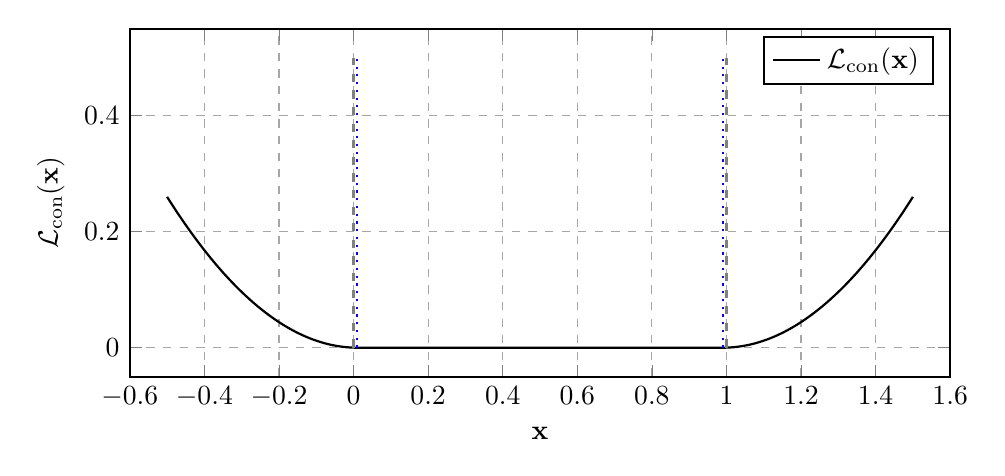
\begin{tikzpicture}
  \begin{axis}[
    width=12cm,
    height=6cm,
    xlabel={$\mathbf{x}$},
    ylabel={$\mathcal{L}_{\mathrm{con}}(\mathbf{x})$},
    grid=major,
    grid style={dashed,gray!70},
    legend style={at={(0.98,0.98)},anchor=north east},
    domain=-0.5:1.5,
    samples=500,
    thick,
    % Automatic spacing like matplotlib margins
    enlarge x limits=0.05,
    enlarge y limits=0.1,
    ]

    % Main function plot
    \addplot [
      color=black,
    ]
    {(1/(1 + exp(-(-((x - 0.01)/0.0025)))) * (0.01 - x)
      + 1/(1 + exp(-((x - 0.99)/0.0025))) * (x - 0.99))^2};
    \addlegendentry{$\mathcal{L}_{\mathrm{con}}(\mathbf{x})$}

    % Vertical reference lines using simple approach
    \addplot[dashed, gray, forget plot] coordinates {(0,0) (0,0.5)};
    \addlegendentry{$a = 0$}

    \addplot[dashed, gray, forget plot] coordinates {(1,0) (1,0.5)};
    \addlegendentry{$b = 1$}

    \addplot[dotted, blue, forget plot] coordinates {(0.01,0) (0.01,0.5)};
    \addlegendentry{$a + \delta$}

    \addplot[dotted, blue, forget plot] coordinates {(0.99,0) (0.99,0.5)};
    \addlegendentry{$b - \delta$}
  \end{axis}
\end{tikzpicture}